% \iffalse meta-comment
% !TEX program  = pdfLaTeX
%<*internal>
\iffalse
%</internal>
%<*readme>
```
----------------------------------------------------------------
cesenaexam --- class file to typeset exams
E-mail: alexpacini90@gmail.com
Released under the LaTeX Project Public License v1.3c or later
See http://www.latex-project.org/lppl.txt
Contributions to this repository as pull requests are welcome!
----------------------------------------------------------------
```

This LaTeX document class has been designed to typeset exams.
To make the ```.cls``` from the ```.dtx``` one, just run
```make```.
Read the manual for more informations.

The processed files ready to be included can be downloaded from
the following links:

[Download cesenaexam Manual](https://alexpacini.github.io/cesenaexam/build/cesenaexam.pdf)

[Download cesenaexam Example](https://alexpacini.github.io/cesenaexam/build/cesenaexam_example.pdf)

<a href="https://alexpacini.github.io/cesenaexam/build/cesenaexam.cls" download="cesenaexam.cls">Download cesenaexam Class File</a>

To use the class file, just drop it in the same folder as the ```.tex``` source file and use ```cesenaexam``` in the
```\documentclass[a4paper, 10pt]{cesenaexam}``` or download the last published version from the archive below.

## Tag Archive
[cesenaexam v0.2](https://github.com/alexpacini/cesenaexam/archive/v0.2.zip)

%</readme>
%<*internal>
\fi
\def\nameofplainTeX{plain}
\ifx\fmtname\nameofplainTeX\else
  \expandafter\begingroup
\fi
%</internal>
%<*install>
\input docstrip.tex
\keepsilent
\askforoverwritefalse
\preamble
----------------------------------------------------------------
cesenaexam --- class file to typeset exams
E-mail: alexpacini90@gmail.com
Released under the LaTeX Project Public License v1.3c or later
See http://www.latex-project.org/lppl.txt
Contributions to this repository as pull requests are welcome!
----------------------------------------------------------------

This LaTeX document class has been designed to typeset exams.
To make the .cls from the .dtx one, just run
```make```.

\endpreamble
\postamble

Copyright (C) 2017 by Alex Pacini <alexpacini90@gmail.com>

This work may be distributed and/or modified under the
conditions of the LaTeX Project Public License (LPPL), either
version 1.3c of this license or (at your option) any later
version.  The latest version of this license is in the file:

http://www.latex-project.org/lppl.txt

This work is "maintained" (as per LPPL maintenance status) by
Alex Pacini.

This work consists of the file  cesenaexam.dtx
and the derived files           cesenaexam.ins,
                                cesenaexam.pdf and
                                cesenaexam.cls.

\endpostamble
\usedir{tex/latex/cesenaexam}
\generate{
  \file{\jobname.cls}{\from{\jobname.dtx}{class,classpackage}}
}
\generate{
  \file{\jobname.sty}{\from{\jobname.dtx}{package,classpackage}}
}
%</install>
%<install>\endbatchfile
%<*internal>
\usedir{source/latex/cesenaexam}
\generate{
  \file{\jobname.ins}{\from{\jobname.dtx}{install}}
}
\nopreamble\nopostamble
\usedir{doc/latex/cesenaexam}
\generate{
  \file{README.md}{\from{\jobname.dtx}{readme}}
}
\ifx\fmtname\nameofplainTeX
  \expandafter\endbatchfile
\else
  \expandafter\endgroup
\fi
%</internal>
%<*class>
\NeedsTeXFormat{LaTeX2e}
\ProvidesClass{cesenaexam}[2017/08/03 - v0.2 Cesena Exam]
\def\cesenaexamversion{0.2}
%</class>
%<*package>
\NeedsTeXFormat{LaTeX2e}
\ProvidesPackage{cesenaexam}[2017/08/03 - v0.2 Cesena Exam]
\def\cesenaexamversion{0.2}
%</package>
%<*driver>
\documentclass{ltxdoc}

\makeatletter% Do not index foreign macros: tex.stackexchange.com/questions/46085
\def\SpecialMainIndex#1{%
\@bsphack
\immediate\write\@auxout{%
\global\noexpand\expandafter\let\noexpand\csname MAIN:\noexpand\string\string#1\endcsname\noexpand\@empty}%
\SpecialIndex@{#1}{\encapchar main}\@esphack}
\def\SpecialIndex#1{%
\@bsphack
   \expandafter\ifx\csname MAIN:\string#1\endcsname\@empty
   \special@index{\expandafter\@gobble
                                      \string#1\actualchar
      \string\verb\quotechar*\verbatimchar\string#1\verbatimchar}%
   \fi
    \@esphack}
\makeatother

\usepackage[T1]{fontenc}
\usepackage[utf8]{inputenc}
%\usepackage{lmodern}
\usepackage[numbered]{hypdoc}
\usepackage{booktabs}
\usepackage{amsfonts, amssymb, amsmath, textcomp, gensymb, mathtools}
\interdisplaylinepenalty=2500
\usepackage{array}
\usepackage{url}
\usepackage{microtype, datetime}
\usepackage{color, soul}
\let\oldsection\section
\let\oldmaketitle\maketitle
\usepackage{\jobname}
\let\section\oldsection
\let\maketitle\oldmaketitle
\EnableCrossrefs
\CodelineIndex
\RecordChanges
\begin{document}
  \DocInput{\jobname.dtx}
\end{document}
%</driver>
% \fi
%
% \def\fileversion{v0.2}
% \def\filedate{2017/08/03}
%
%\title{^^A
%  \textsf{cesenaexam} --- class file to typeset exams\thanks{^^A
%    This file describes version \fileversion, last revised \filedate.^^A
%  }^^A
%}
%\author{^^A
%  Alex Pacini\thanks{E-mail: alexpacini90@gmail.com}^^A
%}
%\date{Released \filedate}
%
%\maketitle
%\tableofcontents
%
%\changes{v0.2}{2017/08/03}{First public release}
%
% \section{How to make}
% This class is also provided with a Makefile and an example document.
%
% Just execute the Makefile with \verb|make| and the class file \verb|cesenaexam.cls|, the package file \verb|cesenaexam.sty|, this manual \verb|cesenaexam.pdf| and the example document \verb|cesenaexam_example.pdf| will be produced.
%
% \section{The cesenaexam document class}
% \verb|\documentclass[a4paper, 10pts]{cesenaexam}|\\
% \newline
% The document class for the \texttt{cesenaexam}, which has few additional optional arguments listed in the following:
% \begin{itemize}
% \item \oarg{boxed}: Draws boxes around blocks.
%   The red box is the tikz bounding box, the black one is the minipage bounding box.
%   Useful for the layout of the page.
% \item \oarg{times}: Sets a times font.
% \item \oarg{noversion}: Hides the footer.
% \item \oarg{left=2cm, right=2cm, top=2.5cm, bottom=2.5cm}: Set the page margins using the geometry package, the defaults are indicated here in the options.
% \end{itemize}
%
%\section{The cesenaexam package}
% \verb|\usepackage{cesenaexam}|\\
% \newline
% \noindent \textcolor{red}{\bfseries Not intended to be used with the class which already defines all the macros}
%
% All the macros are defined also without the class in a standalone package, which is used to make this manual.
% There could be other uses, but those are not guaranteed.
%
%\StopEventually{^^A
%\PrintChanges
%\PrintIndex
%}
%
% \iffalse
%<*classpackage>
% \fi
% 
% \section[Class and package settings and definitions]{{\color{red}Class} and {\color{blue}package} settings and definitions}
%
% In both {\color{red}\verb|cesenaexam.cls|} and {\color{blue}\verb|cesenaexam.sty|}.
%    \begin{macrocode}
%% Custom options
\RequirePackage{etoolbox}
%% I decided to use the etoolbox ifbool because the if else fi
%% has issues with docstrip and needs a dirty hack
%% tex.stackexchange.com/questions/162762
%% No version option
\newbool{exam@version}\booltrue{exam@version}
%% Box the blocks option
\newbool{exam@boxed}\boolfalse{exam@boxed}
%% Times font option
\newbool{exam@times}\boolfalse{exam@times}
%    \end{macrocode}
%\iffalse
%</classpackage>
%<*class>
%\fi
% \noindent
% Only in {\color{red}\verb|cesenaexam.cls|}.
%    \begin{macrocode}
%% No version option
\DeclareOption{noversion}{\boolfalse{exam@version}}
%% Box the blocks option
\DeclareOption{boxed}{\booltrue{exam@boxed}}
%% Times font option
\DeclareOption{times}{\booltrue{exam@times}}
%% This class extends the article class
%% Read all the documentclass options; pass them to article,
\DeclareOption*{\PassOptionsToClass{\CurrentOption}{article}}
\ProcessOptions \relax
%%
\LoadClass{article}
%%
\RequirePackage{pgfkeys}
\RequirePackage{pgfopts}
%%
%% Options to pass to geometry using pgfopts
\pgfkeys{
 /myexamgeometry/.is family, /myexamgeometry,
 left/.default = 2cm,
 right/.default = 2cm,
 top/.default = 2.5cm,
 bottom/.default = 2.5cm,
 left/.store in =\exam@geometryleft,
 right/.store in =\exam@geometryright,
 top/.store in =\exam@geometrytop,
 bottom/.store in =\exam@geometrybottom,
 left, right, bottom, top,
}
\ProcessPgfOptions{/myexamgeometry}
%%
%% Page layout, check if the boxed option is used to load
%% geometry with the showframe option
\ifbool{exam@boxed}{%
\RequirePackage[showframe,%
left=\exam@geometryleft, right=\exam@geometryright,%
top=\exam@geometrytop,bottom=\exam@geometrybottom]{geometry}%
}{%
\RequirePackage[left=\exam@geometryleft, right=\exam@geometryright,%
top=\exam@geometrytop, bottom=\exam@geometrybottom]{geometry}%
}
%%
%% Set the times font if the option is times
\ifbool{exam@times}{%
\RequirePackage{newtxtext,newtxmath}%
}{}
%    \end{macrocode}
%\iffalse
%</class>
%<*classpackage>
%\fi
% In both {\color{red}\verb|cesenaexam.cls|} and {\color{blue}\verb|cesenaexam.sty|}.
%    \begin{macrocode}
%% Loading graphicx before tikz removes a 
%% strange issue with the \graphicspath
\RequirePackage[pdftex]{graphicx}
%% Tikz and circuitikz
\RequirePackage{tikz}
\RequirePackage[betterproportions]{circuitikz}
\usetikzlibrary{arrows.meta,arrows,intersections,%
positioning,fit,calc,through,babel}
\usetikzlibrary{decorations.pathmorphing,backgrounds}
%% Some settings for Tikz
\tikzset{switcharc/.style={draw, thick, >=stealth},
    every picture/.append style={tight background,%
    baseline={([yshift=-1em] current bounding box.north)}}}
%    \end{macrocode}
%\iffalse
%</classpackage>
%<*class>
%\fi
% Only in {\color{red}\verb|cesenaexam.cls|}.
%    \begin{macrocode}
%% Set the Header
\RequirePackage{fancyhdr}
\renewcommand{\headrulewidth}{0pt}
\setlength{\headheight}{25pt} 
\addtolength{\headheight}{\baselineskip}
\fancypagestyle{plain}{
\fancyhead[C]{
\ifbool{exam@boxed}{%
\tikzset{every picture/.style={framed, tight background},%
background rectangle/.style={draw=red}}%
}{}
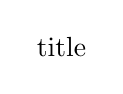
\begin{tikzpicture}
\node (header) [align=center] at (0,0) {\@title};
\end{tikzpicture}%
}%
\ifbool{exam@version}{%
\fancyfoot[L]{{\it Proudly made with} \LaTeX}%
\fancyfoot[R]{CesenaExam v\cesenaexamversion { }- {\it A. Pacini}}%
}{}
}
\pagestyle{plain}
%    \end{macrocode}
%\iffalse
%</class>
%<*classpackage>
%\fi
% In both {\color{red}\verb|cesenaexam.cls|} and {\color{blue}\verb|cesenaexam.sty|}.
%    \begin{macrocode}
%% Redefine the section to have bigger font and to be
%% delimited between two lines
\RequirePackage{titlesec}
\newcommand{\sectionfont}{\Large}
\renewcommand\thesection{\bfseries \arabic{section}} 
\titleformat{\section}
    {\titlerule     
     \vspace{0.5ex}%
     \sectionfont}
    {\thesection}{1em}
    {\sectionfont \bfseries}[\titlerule]
%% Redefine the enumerate item to be bold
\renewcommand\labelenumi{\bfseries\theenumi.}
%% Options for the titlebox processed from the
%% maketitle optional arguments
\pgfkeys{
 /mytitlebox/.is family, /mytitlebox,
 textboxheight/.default = 0.6cm,
 whiteboxheight/.default = 1cm,
 textboxheight/.store in = \minheighttext@title,
 whiteboxheight/.store in = \minwhiteboxheight@title,
 textboxone/.default = {\relax},
 textboxtwo/.default = {\relax},
 textboxthree/.default = {\relax},
 textboxfour/.default = {\relax},
 textboxone/.store in = \textboxone@title,
 textboxtwo/.store in = \textboxtwo@title,
 textboxthree/.store in = \textboxthree@title,
 textboxfour/.store in = \textboxfour@title,
 %% Executing them to assign the default value
 %% (Tikz manual 82.3.2 or tex.stackexchange.com/questions/85754)
 textboxheight, whiteboxheight, textboxone,
 textboxtwo, textboxthree, textboxfour,
}
%    \end{macrocode}
%\iffalse
%</classpackage>
%\fi

%\iffalse
%<*internal>
\iffalse
%</internal>
%<*comment>
%% Just two example definition to be copied and pasted
%
%% Example definition of a macro with starred version, using describe macro:
%
%\DescribeMacro{\macroname}
% Usage: \verb|\macroname|\marg{mandatory 1}\marg{mandatory 2} \\
% Description.\\
% 
%\DescribeMacro{\macroname*}
% Usage: \verb|\macroname*|\marg{mandatory 1}\marg{mandatory 2} \\
% Description.\\
%
% Definition of \cs{macroname} and \cs{macroname*}:
%\DoNotIndex{\def,\@ifstar} ^^A Not really needed with the modified index macro in the doc document (see above)
%    \begin{macrocode} ^^A The four spaces are mandatory!
%% Comment
\def\macroname{\@ifstar\macro@name\macro@@name}
\def\macro@name#1#2{\relax}
\def\macro@@name#1#2{\relax}
%    \end{macrocode}
%
%% Example definition of a macro:
% 
%\begin{macro}{\macroname}
% Usage: \verb|\macroname|\marg{mandatory 1}\marg{mandatory 2} \\
% Description.\\
%
% Definition of \cs{macroname}:
%\DoNotIndex{\def} ^^A Not really needed with the modified index macro in the doc document (see above)
%^^A The four spaces are mandatory!
%    \begin{macrocode}
%% Comment
\def\macroname#1#2{\relax}
%    \end{macrocode}
%\end{macro}
%</comment>
%<*internal>
\fi
%</internal>
%\fi

%\iffalse
%<*classpackage>
%\fi
% \section{Defined Macros} \indent
%
%\DescribeMacro{\examsection}
% Usage: \verb|\examsection|\marg{bold title}\marg{italic text} \\
% Prints the title between two lines \textbf{with} numbering.\\
% 
%\DescribeMacro{\examsection*}
% Usage: \verb|\examsection*|\marg{bold title}\marg{italic text} \\
% Prints the title between two lines \textbf{without} numbering.\\
%
% Definition of \cs{examsection} and \cs{examsection*}:
%\DoNotIndex{\def,\@ifstar,\@examsection,\@@examsection,\textmd,\textit,\noindent,\section}
%    \begin{macrocode}
%% Define examsection and examsection*
\def\examsection{\@ifstar\@examsection\@@examsection}
\def\@examsection#1#2{\section*{#1 \textmd{(\textit{#2})}}\noindent}
\def\@@examsection#1#2{\section{#1 \textmd{(\textit{#2})}}\noindent}
%    \end{macrocode}
%
%\begin{macro}{\boxempty}
% Usage: \verb|\boxempty| $\to$ \boxempty \\
% Prints an empty box.
%
% Definition of \verb|\boxempty|:
%\DoNotIndex{\newcommand,\square,\;}
%    \begin{macrocode}
%% Definition of empty tick box
\newcommand{\boxempty}{$ \square \;$}
%    \end{macrocode}
%\end{macro}
%
%\begin{macro}{\boxcheck}
% Usage: \verb|\boxcheck| $\to$ \boxcheck \\
% Prints a black or \textit{checked} box.
%
% Definition of \verb|\boxcheck|:
%\DoNotIndex{\newcommand,\square,\;}
%    \begin{macrocode}
%% Definition of empty tick box
\newcommand{\boxcheck}{$ \blacksquare \;$}
%    \end{macrocode}
%\end{macro}
%
%\begin{macro}{\examparts}
% Usage: \verb|\examparts|\marg{}
%\begin{verbatim}
%\examparts{\bfseries Parts done: \hspace{1cm}%
%   E1 \boxempty \hspace{1cm}%
%   E2 \boxempty \hspace{1cm}%
%   D \boxempty}
% \end{verbatim}
% Used to include the checkboxes in \cs{maketitle} by passing the code to the \cs{examparts\{\}} macro.
% It is internally assigned to the variable \cs{ex@parts}.
% 
% Definition of \verb|\examparts{}|:
%    \begin{macrocode}
%% Assigns to ex@parts what is passed to the function examparts{}.
%% Works similarly similarly to author{}
\def\examparts#1{\def\ex@parts{#1}}
%    \end{macrocode}
%\end{macro}
%
%\DescribeMacro{\maketitle}
% Usage: \cs{maketitle}\oarg{opt. args}\marg{Surname}\marg{Name}\marg{Id}\marg{Signature}\marg{N} \\
% Redefines the \cs{maketitle}.\\
% The mandatory arguments label the text (or top) boxes, where the last one used to give the exam type using one char or number.
% It is also possible to give optional arguments:
% \begin{itemize}
% \item \oarg{textboxheight=0.6cm, whiteboxheight=1cm}: To set the height of the textboxes (\verb|textboxheight|) and of the whiteboxes (\verb|whiteboxheight|), the defaults are indicated here in the options;
% \item \oarg{textboxone={Guglielmo}, textboxtwo={Marconi}, textboxthree={000},%\\ textboxfour={Signature.pdf}}: To fill the whiteboxes, default are empty.
% \end{itemize}
% A usage example is:
%\begin{verbatim}
%\maketitle[textboxheight=0.6cm, whiteboxheight=1cm,%
%   textboxone={Guglielmo}, textboxtwo={Marconi}, textboxthree={00000000},%
%   textboxfour={
\includegraphics[width=3cm]{Guglielmo_Marconi_Signature}}]%
%   {Cognome}{Nome}{Matricola}{Firma}{1}
% \end{verbatim}
% 
%\DescribeMacro{\maketitle*}
% Not implemented at the moment.\\
%
% Definition of \cs{maketitle} and \cs{maketitle*}:
%\DoNotIndex{\def,\@ifstar} ^^A Not really needed with the modified index macro in the doc document (see above)
%    \begin{macrocode}
%% Redefine maketitle
%% Just for a future starred version
\def\maketitle{\@ifstar\make@@title\make@title}%
%% Define the unstarred version maketitle (make@title)
\newcommand\make@title[6][]{%
 \pgfkeys{/mytitlebox, #1}%
 \make@@@title{#2}{#3}{#4}{#5}{#6}}%
%% Define the common command
\def\make@@@title#1#2#3#4#5{%
\ifbool{exam@boxed}{%
\tikzset{every picture/.append style={framed},%
background rectangle/.style={draw=red}}}{}%
\begin{center}%
\begin{tikzpicture}%
\pgfmathsetmacro{\boxlen}{(\textwidth-1.6cm)/4}%
\pgfmathsetmacro{\lastboxlen}{\textwidth - 4*\boxlen - 1mm}%
\node (surname) [draw, align=center, minimum width=\boxlen,%
minimum height = \minheighttext@title] at (0,0) {\bf #1};%
\node (surname box) [draw, anchor=north, minimum width=\boxlen,%
minimum height = \minwhiteboxheight@title] at%
($(surname.south)+(0,\pgflinewidth)$) {\textboxone@title};%
\node (name) [draw, align=center, right=0 and -\pgflinewidth of surname,%
minimum width=\boxlen, minimum height = \minheighttext@title] {\bf #2};%
\node (name box) [draw, anchor=north, minimum width=\boxlen,%
minimum height = \minwhiteboxheight@title] at%
($(name.south)+(0,\pgflinewidth)$) {\textboxtwo@title};%
\node (id) [draw, align=center, right=0 and -\pgflinewidth of name,%
minimum width=\boxlen, minimum height = \minheighttext@title] {\bf #3};%
\node (id box) [draw, anchor=north, minimum width=\boxlen,%
minimum height = \minwhiteboxheight@title] at%
($(id.south)+(0,\pgflinewidth)$) {\textboxthree@title};%
\node (signature) [draw, align=center, right=0 and -\pgflinewidth of id,%
minimum width=\boxlen, minimum height = \minheighttext@title] {\bf #4};%
\node (signature box) [draw, anchor=north, minimum width=\boxlen,%
minimum height = \minwhiteboxheight@title] at%
($(signature.south)+(0,\pgflinewidth)$) {\textboxfour@title};%
%%
\pgfmathsetmacro{\minheighttypebox}{\minheighttext@title +%
\minwhiteboxheight@title}%
\node (examtype) [draw, align=center, anchor=north west,%
minimum width=\lastboxlen, minimum height = \minheighttypebox] at%
($(signature.north east)+(-\pgflinewidth,0)$) {\Huge \bfseries #5};%
\node (checkboxes) [align=left, anchor=north west] at%
(surname box.south west) {\ex@parts};%
\end{tikzpicture}%
\end{center}%
}
%    \end{macrocode}
%
%\begin{macro}{\examtwoblocks}
% Usage: \verb|\examtwoblocks|\marg{B1 length}\marg{B2 length}\marg{B1}\marg{B2} \\
% Defines the macro \cs{examtwoblocks}.\\
% The mandatory arguments are the lenght of the first block and of the second block, and their content, respectively.
% They two boxes are vertically aligned to their centre.
%
% Definition of \cs{examtwoblocks}:
%\DoNotIndex{\def} ^^A Not really needed with the modified index macro in the doc document (see above)
%    \begin{macrocode}
%% Macro for two blocks centre aligned
\def\examtwoblocks#1#2#3#4{%
\noindent%
\begin{minipage}[c]{#1}\flushleft#3\end{minipage}%
\hfill%
\begin{minipage}[c]{#2}#4\end{minipage}
\par\vspace{5mm}\noindent%
}
\def\examtwoblocks@box#1#2#3#4{%
\noindent%
\tikzset{every picture/.append style={framed},
    background rectangle/.style={draw=red}}%
\let\bak@fboxsep\fboxsep%
\def\fboxsep{0pt}%
\fbox{\begin{minipage}[c]{#1}\flushleft#3\end{minipage}}%
\hfill%
\fbox{\begin{minipage}[c]{#2}#4\end{minipage}}%
\let\fboxsep\bak@fboxsep%
\par\vspace{5mm}\noindent%
}
\ifbool{exam@boxed}{%
\renewcommand{\examtwoblocks}{\examtwoblocks@box}}{}
%    \end{macrocode}
%\end{macro}
%
%
%\begin{macro}{\examtwoblockstop}
% Usage: \verb|\examtwoblockstop|\marg{B1 length}\marg{B2 length}\marg{B1}\marg{B2} \\
% Defines the macro \cs{examtwoblockstop}.\\
% The mandatory arguments are the lenght of the first block and of the second block, and their content, respectively.
% They two boxes are vertically aligned to their top, which is useful if used inside an itemize or an enumerate environment.
%
% Definition of \cs{examtwoblockstop}:
%\DoNotIndex{\def} ^^A Not really needed with the modified index macro in the doc document (see above)
%    \begin{macrocode}
%% Macro for two blocks top aligned
\def\examtwoblockstop#1#2#3#4{%
\noindent%
\begin{minipage}[t]{#1}\flushleft#3\end{minipage}%
\hfill%
\begin{minipage}[t]{#2}\flushright#4\end{minipage}%
}
\def\examtwoblockstop@box#1#2#3#4{%
\noindent%
\tikzset{every picture/.append style={framed},
    background rectangle/.style={draw=red}}%
\let\bak@fboxsep\fboxsep%
\def\fboxsep{0pt}%
\fbox{\begin{minipage}[t]{#1}\flushleft#3\end{minipage}}%
\hfill%
\fbox{\begin{minipage}[t]{#2}\flushright#4\end{minipage}}%
\let\fboxsep\bak@fboxsep%
}
\ifbool{exam@boxed}{%
\renewcommand{\examtwoblockstop}{\examtwoblockstop@box}}{}
%    \end{macrocode}
%\end{macro}
%
%\begin{macro}{\examoneblocktop}
% Usage: \verb|\examoneblocktop|\marg{B length}\marg{B} \\
% Defines the macro \cs{examoneblock}.\\
% The mandatory arguments are the lenght of the block and its content.
% They box is vertically aligned to its top, which is useful if used inside an itemize or an enumerate environment.
%
% Definition of \cs{examoneblock}:
%\DoNotIndex{\def} ^^A Not really needed with the modified index macro in the doc document (see above)
%    \begin{macrocode}
%% Macro for one block top aligned
\def\examoneblocktop#1#2{%
\noindent%
\begin{minipage}[t]{#1}\flushleft#2\end{minipage}}%
\def\examoneblocktop@box#1#2{%
\noindent%
\tikzset{every picture/.append style={framed},
    background rectangle/.style={draw=red}}%
\let\bak@fboxsep\fboxsep%
\def\fboxsep{0pt}%
\fbox{\begin{minipage}[t]{#1}\flushleft#2\end{minipage}}%
\let\fboxsep\bak@fboxsep%
}
\ifbool{exam@boxed}{%
\renewcommand{\examoneblocktop}{\examoneblocktop@box}}{}
%    \end{macrocode}
%\end{macro}
%
%\iffalse
%</classpackage>
%\fi

%\Finale
